\chapter{Introduction to Verilog}
\label{introductionToVerilog}
\graphicspath{ {./Lab01SimpleVerilog/Fig} }

\section{Outcomes and Objective }

The outcome of this lab is to introduce you to the Quartus II
software, design entry using Verilog and circuit simulation.
Through this process you will achieve the following
learning objectives.
\begin{itemize}
        \itemsep=0em
    \item \Paste{bok:REP_Elfs}
    \item \Paste{bok:REP_Convert}
    \item \Paste{VER:CSA}
    \item \Paste{VER:Logic}
    \item\Paste{HDL:Time}
\end{itemize}

\section{FPGA: Creating a project in Quartus and running a testbench}
In this section you will apply inputs to a 2-input AND gate and
observing the output on a timing diagram.  Since all this activity will
take place in the memory of a computer and not on actual hardware,
it is called a simulation.  To start this process, you will first have to
create a project and add files to it.

\begin{enumerate}
        \def\labelenumi{\arabic{enumi}.}
    \item
        Select an appropriate working directory for your project. I would
        recommend selecting your network drive.

        \begin{enumerate}
                \def\labelenumii{\alph{enumii}.}
            \item
                Create a new folder \emph{lab1},
            \item
                Create another folder within \emph{lab1} called \emph{andgate2},
            \item
                Download \emph{andgate2.v} and \emph{andgate2\_tb.v} from Canvas,
            \item
                Save these files in andgate2 directory.
        \end{enumerate}
    \item
        Start Quartus II.

        \begin{enumerate}
                \def\labelenumii{\alph{enumii}.}
            \item
                If you are prompted by a License Setup choose the free option. You
                may need to restart Quartus if this happens.
        \end{enumerate}
    \item
        Select \emph{File -\textgreater{} New Project Wizard.}
    \item
        In the \textbf{Directory, Name, Top-Level Entity} page of the New
        Project Wizard pop-up:

        \begin{enumerate}
                \def\labelenumii{\alph{enumii}.}
            \item
                To the right of the ``What is the working directory'' box click the
                \ldots{} button,
            \item
                In the Select Folder pop-up, navigate so you can see the andgate2
                directory created in step 1,
            \item
                Select the andgate2 folder, click Select Folder,
            \item
                In the ``What is the name of this project'' field type
                \emph{andgate2}
            \item
                click \emph{Next}.
        \end{enumerate}
    \item
        In the \textbf{Project Type} page of the New Project Wizard pop-up:

        \begin{enumerate}
                \def\labelenumii{\alph{enumii}.}
            \item
                Select the \emph{Empty project} radio button,
            \item
                click \emph{Next}.
        \end{enumerate}
    \item
        In the \textbf{Add Files} page of the New Project Wizard pop-up:

        \begin{enumerate}
                \def\labelenumii{\alph{enumii}.}
            \item
                Click the \ldots{} button to the right of File name,
            \item
                In the Select File pop-up, navigate to, and select,
                \emph{andgate2.v} and \emph{andgate2\_tb.v}, click Open,
            \item
                The file should appear in the window below,
            \item
                Click \emph{Next}
        \end{enumerate}
    \item
        In the \textbf{Family \& Device Settings} page of the New Project
        Wizard pop-up:

        \begin{enumerate}
                \def\labelenumii{\alph{enumii}.}
            \item
                Device family, Family: Cyclone V
            \item
                Package: FBGA
            \item
                Pin Count: 672
            \item
                Speed Grade: 7\_H6
            \item
                Select Specific device selected in `Available devices' list
            \item
                From the list of available devices, select: 5CGXFC5C6F27C7
            \item
                Click Next
        \end{enumerate}
    \item
        In the \textbf{EDA Tool Settings} page of the New Project Wizard
        pop-up:

        \begin{enumerate}
                \def\labelenumii{\alph{enumii}.}
            \item
                In the Simulation row

                \begin{enumerate}
                        \def\labelenumiii{\roman{enumiii}.}
                    \item
                        Tool Name column: ModelSim-Altera
                    \item
                        Formats column: Verilog HDL
                \end{enumerate}
            \item
                Leave other defaults alone
            \item
                Click Next
        \end{enumerate}
    \item
        In the \textbf{Summary} page of the New Project Wizard pop-up:

        \begin{enumerate}
                \def\labelenumii{\alph{enumii}.}
            \item
                Review information,
            \item
                Click Finish.
        \end{enumerate}
    \item
        Back in the main Quartus II window, Click \emph{Tools -\textgreater{}
        Options..}.
    \item
        In the Options pop-up:

        \begin{enumerate}
                \def\labelenumii{\alph{enumii}.}
            \item
                Select \emph{EDA Tool Options} from the Category menu,
            \item
                If the last row, ``ModelSim-Altera'' is blank, click on the \ldots{}
                button at right and navigate to the
                \emph{C:\textbackslash intelFPGA\_lite\textbackslash18.1\textbackslash modelsim\_ase\textbackslash{}},
                select the \emph{win32aloem} folder, the click Select Folder.  Note the software version in
                these instructions
                is 18.1  The version installed on your computer may be different.  If so, the path should be
                the same with the
                exception of the version number.
            \item
                Click Ok.
        \end{enumerate}
    \item
        Click on the Files tab in the \emph{Project Navigator} pane.

        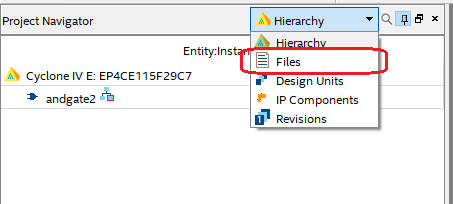
\includegraphics[width=3.9in,height=1.8in]{image1.png}

    \item
        Right click on \emph{andgate2\_tb} in the \emph{Project Navigator}
        pane and select Set as Top-Level entity.
    \item
        Double click on \emph{andgate2}.
    \item
        If you added the Verilog file in the correct directory and included it
        in the project, a Verilog file should pop up on the right.
    \item
        In the main Quartus II window, click on \emph{Processing
        -\textgreater{} Start -\textgreater{} Start Analysis \& Elaboration.}
        This may take some time, so be patient.
    \item
        If you did everything correctly you should

        \begin{enumerate}
                \def\labelenumii{\alph{enumii}.}
            \item
                Notice that andgate\_tb is the new top-level entity in the Hierarchy
                pane. Expand the andgate2\_tb by clicking on the ``\textgreater''
                arrow to see the entities inside it.
            \item
                You should see the following messages in the console area, the
                bottom pane.
        \end{enumerate}
\end{enumerate}

\begin{quote}
    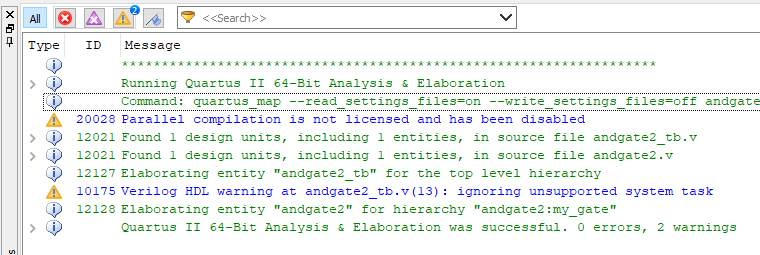
\includegraphics{image2.png}
\end{quote}

\begin{enumerate}
        \def\labelenumi{\arabic{enumi}.}
        \setcounter{enumi}{17}
    \item
        In the main Quartus II window, click \emph{Tools -\textgreater{} Run
        Simulation Tool -\textgreater{} RTL Simulation}. The ModelSim program
        will launch. This may take a few moments, be patient. If you get a
        pop-up Nativelink Error window, then go back, check and fix the
        directory in step 11.
    \item
        In ModelSim, click Simulate -\textgreater{} Start Simulation
    \item
        In the Start Simulation pop-up, expand the \emph{work} library by
        clicking on the ``+'' at left. click on \emph{andgate2\_tb} and click
        \emph{Ok}.
    \item
        In the sim pane, right mouse click on uut and select \emph{Add Wave}.
\end{enumerate}

\begin{quote}
    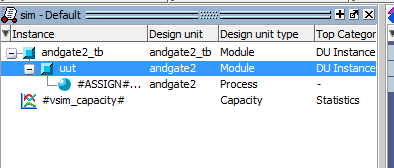
\includegraphics[width=4.10417in,height=1.75in]{image3.png}
\end{quote}

\begin{enumerate}
        \def\labelenumi{\arabic{enumi}.}
        \setcounter{enumi}{21}
    \item
        Choose \emph{Simulate -\textgreater{} Run -\textgreater{} Run 100}.
        You should see inputs and output from andgate2. If you see only a
        small green portion of the waveform on the left margin of the timing
        diagram, you will need to zoom in on the waveform as follows. First
        click somewhere in the timing diagram (area under ``Undocking tool''
        in the image below) and then click on the ``Zoom all tool'' shown in
        following image.
    \item
        \protect\hypertarget{Part_1_Step_23}{}{}Save this waveform as an image
        as follows:

        \begin{enumerate}
                \def\labelenumii{\alph{enumii}.}
            \item
                Undock the Wave pane by clicking the undocking tool icon.
        \end{enumerate}
\end{enumerate}

\begin{quote}
    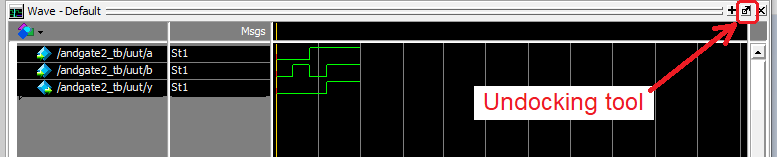
\includegraphics{image4.png}
\end{quote}

\begin{enumerate}
        \def\labelenumi{\alph{enumi}.}
        \setcounter{enumi}{1}
    \item
        Resize the undocked Wave window vertically by grabbing its top edge
        and dragging down. Make the window tall enough to fit all the waves
        with a little room to spare.
\end{enumerate}

\begin{quote}
    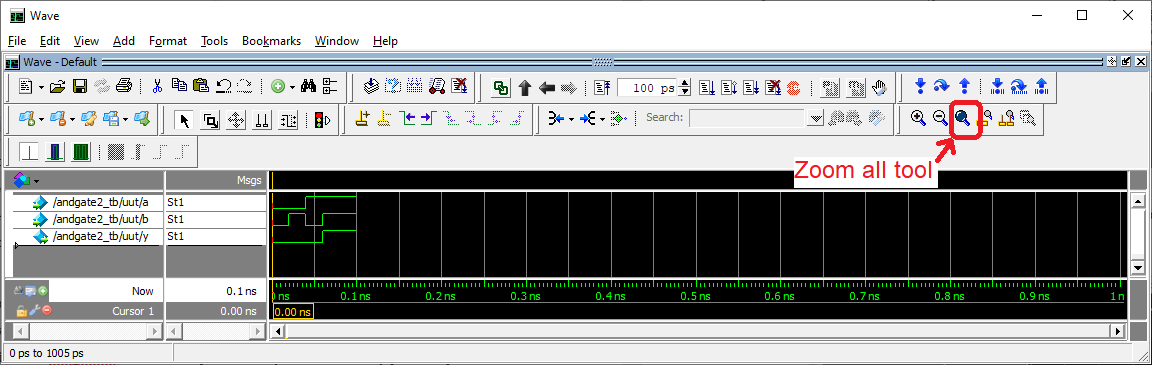
\includegraphics{image5.png}
\end{quote}

\begin{enumerate}
        \def\labelenumi{\alph{enumi}.}
        \setcounter{enumi}{2}
    \item
        Click the Zoom all tool to file the available horizontal space with
        the waveform.
    \item
        Click File -\textgreater{} Export -\textgreater{} Image
\end{enumerate}

\begin{quote}
    If this does not work, you can take a screen shot of the window by
    pressing Alt-Print Screen. The ``Alt'' captures the currently active
    window into the graphics buffer.
\end{quote}

\begin{enumerate}
        \def\labelenumi{\alph{enumi}.}
        \setcounter{enumi}{4}
    \item
        Navigate to your project directory, provide a File name, then click
        Save
    \item
        Exit Modelsim using File -\textgreater{} Quit. Do not save wave
        commands.
\end{enumerate}

\begin{enumerate}
        \def\labelenumi{\arabic{enumi}.}
        \setcounter{enumi}{23}
    \item
        Back in Quartus, close your current project using File -\textgreater{}
        Close Project. Save if needed.
\end{enumerate}

\section{FPGA: Symbolic to Verilog , Timing Diagram, Truth Table}
Write Verilog code to realize the function \emph{f02 = a' + bc'} Note
that this symbolic expression is written using the notation used in
class. This is not a valid Verilog expression.

\begin{enumerate}
        \def\labelenumi{\arabic{enumi}.}
    \item
        Create \textbf{a new project} folder within your \emph{lab1} directory
        called \emph{function02.}
    \item
        Download \emph{function02.v} and \emph{function02\_tb.v} from Canvas
        to the project directory.
    \item
        Create a project for these two files using the steps above.
    \item
        \protect\hypertarget{Part_2_Step_4}{}{}Modify the line of code that
        starts with \emph{assign} to realize the function \emph{f02} shown
        above.
    \item
        Modify \emph{function02\_tb.v} so that \emph{f02} is run through every
        combination of inputs. Assert the inputs in increasing binary
        numbering order starting from 0,0,0 and going to 1,1,1.
    \item
        Perform simulation using the given testbench as described in previous
        steps. You will need to ``run 100'' twice as the simulation is over
        100ns long.
    \item
        \protect\hypertarget{Part_2_Step_7}{}{}Save this waveform as an image
        as done in the previous section. If the waveform is missing, you can
        add it back in using View -\textgreater{} Waveform.
    \item
        \protect\hypertarget{Part_2_Step_8}{}{}From the information in the
        timing diagram, produce a truth table for \emph{f02}. Remember that a
        truth table is an enumeration of every possible input and the
        associated output. Please look at Chapter 2 in the textbook for some
        examples if you are unclear about how to setup a truth table.
\end{enumerate}

\section{FPGA: Verilog to Symbolic, Truth Table, Circuit Diagram}

The Verilog code in the file function03 contains a complete circuit for
\emph{f03}. You will use the Quartus tools to get a timing diagram for
the function and, by looking at the Verilog code, determine the symbolic
form and circuit diagram.

\begin{enumerate}
        \def\labelenumi{\arabic{enumi}.}
    \item
        Create \textbf{a new project} folder within your \emph{lab1} directory
        called \emph{function03.}
    \item
        Download \emph{function03.v} and \emph{function03}\_tb.v from Canvas
        to the project directory.
    \item
        Create a project for these two files using the steps above.
    \item
        Modify \emph{function03\_tb.v} so that \emph{f03} is run through every
        combination of inputs. Assert the inputs in increasing binary
        numbering order starting from 0,0,0 and going to 1,1,1.
    \item
        Perform simulation using this test bench as described in previous
        steps. You will need to ``run 100'' twice as the simulation is over
        100ns long.
    \item
        \protect\hypertarget{Part_3_Step_6}{}{}Save this waveform as an image,
        but with the following changes.

        \begin{enumerate}
                \def\labelenumii{\alph{enumii}.}
            \item
                Resize the area containing the names of the signals by grabbing the
                right vertical bar of the name area and moving it right.
            \item
                Re-order the waves so that f03 is lowest. Do this by grabbing the
                name ``/function03\_tb/uut/f03 and moving it below all the other
                signals.
            \item
                Color the intermediate signals (p1, p2, p4, p7) yellow by right
                clicking on them, selecting properties. In the View tab of the Wave
                Properties pop-up, click the Colors\ldots{} button for Wave Color
                and choose Yellow, click Close, then OK.
            \item
                Change the color of \emph{f03} to red.
        \end{enumerate}
    \item
        \protect\hypertarget{Part_3_Step_7}{}{}From the information in the
        timing diagram, produce a truth table.
    \item
        \protect\hypertarget{Part_3_Step_8}{}{}From the information in
        \emph{function03.v} draw the circuit diagram for \emph{f03}.
    \item
        \protect\hypertarget{Part_3_Step_9}{}{}From the information in
        \emph{function03.v} write down the symbolic form for \emph{f03}.
\end{enumerate}

\section{FPGA: Circuit Diagram to Verilog, Symbolic, Truth Table}

Write Verilog code to realize the function \emph{f04} shown in the
circuit diagram below.

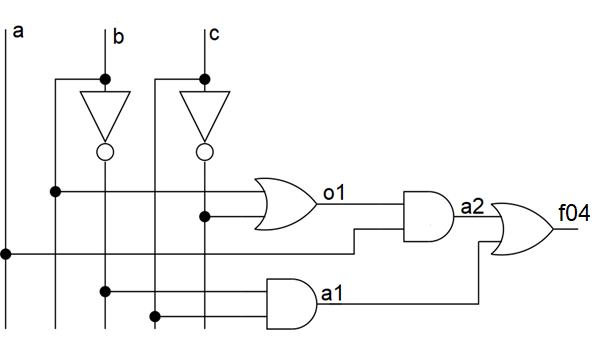
\includegraphics{image6.png}

\begin{enumerate}
        \def\labelenumi{\arabic{enumi}.}
    \item
        Create \textbf{a new project} folder within your \emph{lab1} directory
        called \emph{function04.}
    \item
        Download \emph{function04.v} and \emph{function04}\_tb.v from Canvas
        to the project directory.
    \item
        Create a project for these two files using the steps above.
    \item
        \protect\hypertarget{Part_4_Step_4}{}{}Modify \emph{function04.v} by
        writing an assignment statement for each of \emph{o1}, \emph{a1},
        \emph{a2}, and \emph{f04}.
    \item
        Modify \emph{function04\_tb.v} so that \emph{f04} is run through every
        combination of inputs. Assert the inputs in increasing binary
        numbering order starting from 0,0,0 and going to 1,1,1.
    \item
        Perform simulation using this test bench as described in previous
        steps. You will need to ``run 100'' twice as the simulation is over
        100ns long.
    \item
        \protect\hypertarget{Part_4_Step_7}{}{}Save this waveform as an image
        as done in a previous section. Color intermediate signals (01, a1, a2)
        yellow and output red.
    \item
        \protect\hypertarget{Part_4_Step_8}{}{}From the information in the
        timing diagram, produce a truth table.
\end{enumerate}

\section{Turn in}

Make a record of your response to numbered items below and turn them in
a single copy as your team's solution on Canvas using the instructions
posted there. Include the names of both team members at the top of your
solutions. Use complete English sentences to introduce what each of the
following listed items (below) is and how it was derived.

\subsubsection{FPGA: Creating a project in Quartus and running a testbench}
\begin{itemize}
    \item \protect\hyperlink{Part_1_Step_23}{Step 23} Timing diagram of AND gate
\end{itemize}

\subsubsection{FPGA: Symbolic to Verilog , Timing Diagram, Truth Table}
\begin{itemize}
    \item \protect\hyperlink{Part_2_Step_4}{Step 4} Verilog code for \emph{f02}
    \item \protect\hyperlink{Part_2_Step_7}{Step 7} Timing diagram of \emph{f02}
    \item \protect\hyperlink{Part_2_Step_8}{Step 8} Truth table of \emph{f02}
\end{itemize}

\subsubsection{FPGA: Verilog to Symbolic, Truth Table, Circuit Diagram}
\begin{itemize}
    \item \protect\hyperlink{Part_3_Step_6}{Step 6} Timing diagram of \emph{f03}
    \item \protect\hyperlink{Part_3_Step_7}{Step 7} Truth table of \emph{f03}
    \item \protect\hyperlink{Part_3_Step_8}{Step 8} Circuit    Diagram of \emph{f03}
    \item \protect\hyperlink{Part_3_Step_9}{Step 9} Symbolic form of \emph{f03}
\end{itemize}

\subsubsection{FPGA: Circuit Diagram to Verilog, Symbolic, Truth Table}
\begin{itemize}
    \item \protect\hyperlink{Part_4_Step_4}{Step 4} Just the 4 Verilog assign statement
        for \emph{o1}, \emph{a1}, \emph{a2}, and \emph{f04}.
    \item \protect\hyperlink{Part_4_Step_7}{Step 7} Timing diagram of \emph{f04}
    \item \protect\hyperlink{Part_4_Step_8}{Step 8} Truth table of \emph{f04}
\end{itemize}
